

\section{Πρόσθεση στο Δυαδικό}

Η πρόσθεση δυο δυαδικών ψηφίων x , y έχει αποτέλεσμα το άθροισμα των δυο αυτών ψηφίων sum καθώς και το κρατούμενο εξόδου c\_out, όπως ακριβώς ισχύει και με την άθροιση στο δεκαδικό σύστημα , και ορίζεται ως :\\


% Table Half Adder
%------------------------------------------
\begin{table}[ht]
\centering
 \begin{tabular}{||c c | c c||} 
 \hline
 x & y & sum & c\_out \\ [0.5ex] 
 \hline\hline
 0 & 0 & 0 & 0 \\ 
 \hline
 0 & 1 & 1 & 0 \\
 \hline
 1 & 0 & 1 & 0 \\
 \hline
 1 & 1 & 0 & 1 \\
 \hline
\end{tabular}
\caption{Half Adder Truth Table}
\label{table:1}
\end{table}


% Figure
% HA-Schematic
%--------------------------------------------
\begin{figure}[ht]
\centering
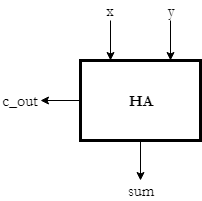
\includegraphics[scale=0.6]{HA.png}
\caption{Half-Adder schematic}
\label{HASchematic}
\end{figure}


Το παραπάνω σύστημα ονομάζεται ημιαθροιστής ή Half-Adder (HA) , έχει δυο εισόδους τις x και y και δυο εξόδους τις c\_out και sum και οι έξοδοι σύμφωνα με τον παραπάνω πίνακα αληθείας περιγράφονται από τις παρακάτω συναρτήσεις άλγεβρας Μπουλ :\\
\begin{equation}
\begin{split}
    sum &= x \oplus y \\ 
    c\_out &= x * y
\end{split}
\end{equation}\\



Από τον ημιαθροιστής δομείται ο πλήρης αθροιστής ή Full-Adder (FA) με τρεις εισόδους x, y, z , δυο εξόδους sum και c\_out και λειτουργία αντίστοιχη του FA με την διαφορά πως ο FA προσθέτει τρία δυαδικά ψηφιά \\
\begin{table}[ht]
\centering
 \begin{tabular}{||c c c | c c||} 
 \hline
 x & y & z & sum & c\_out \\ [0.5ex] 
 \hline\hline
 0 & 0 & 0 & 0 & 0 \\ 
 \hline
 0 & 0 & 1 & 1 & 0 \\
 \hline
 0 & 1 & 0 & 1 & 0 \\
 \hline
 0 & 1 & 1 & 0 & 1 \\
 \hline
 1 & 0 & 0 & 1 & 0 \\ 
 \hline
 1 & 0 & 1 & 0 & 1 \\
 \hline
 1 & 1 & 0 & 0 & 1 \\
 \hline
 1 & 1 & 1 & 1 & 1 \\
 \hline
\end{tabular}
\caption{Full Adder Truth Table}
\label{table:2}
\end{table}
\\
% Figure
% FA-Schematic
%--------------------------------------------
\begin{figure}[ht]
\centering
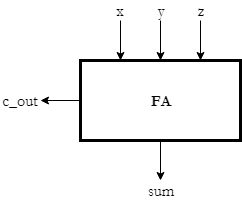
\includegraphics[scale=0.6]{FA.png}
\caption{Full-Adder schematic}
\label{FASchematic}
\end{figure}
\\
και οι εξισώσεις των εξόδων είναι :
\\
\begin{equation}
\begin{split}
    sum &= x \oplus y \oplus z \\
    c_out &= ( x * y ) + ( x * z ) + ( z * y )
\end{split}
\end{equation}

\clearpage


% 
%------------------------------------------------------------
\subsection{Πρόσθεση δυαδικών αριθμών}

Η πρόσθεση δυο δυαδικών αριθμών A και Β των n δυαδικών ψηφίων το κάθε ένα είναι 
μια επέκταση της πρόσθεσης μεταξύ ψηφίων που παρουσιάστηκε προηγουμένως τροφοδοτώντας 
το κρατούμενο εισόδου των προηγούμενων σημαντικών ψηφίων στην είσοδο του πλήρη αθροιστή 
των επομένων .
\\
% Figure
% FA-Schematic
%--------------------------------------------
\begin{figure}[ht]
\centering
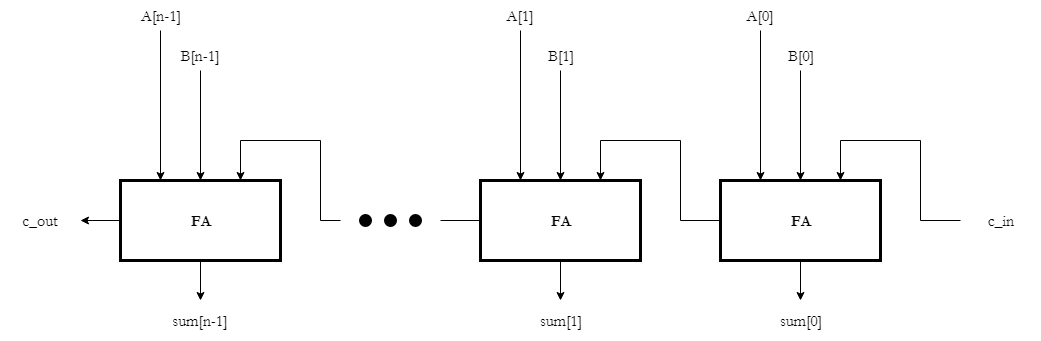
\includegraphics[width=\textwidth]{IntAdder.png}
\caption{Integer-Adder schematic}
\label{IntegerAdderSchematic}
\end{figure}
\\



